
\chapter{Popular Data Processing Frameworks for Java \label{chapter:frameworks}}

In this chapter, we show basic features of chosen frameworks
that are used for manipulating data.
We focus on the basic features relevant for the data lineage
and ignore most of their advanced features.

We show data lineage basic examples of how data can be loaded or stored by Java application
and how sources and sinks are identified, as this is the main topic of our work.

All frameworks that are using database, would work with the example
of storing and loading objects of the class \Code{DatabaseValue} in the Listing \ref{code:model}
from database structured as in Table \ref{code:db}.

\InsertCode{h}{code/model}

TODO RE model databaze:
\begin{lstlisting}[caption={Example of database}, label={code:db}]
TABLE T
ID  | VALUE
1   | A
2   | B
... | ...
\end{lstlisting}







\section{JDBC API \label{frameworks:jdbc}}

For accessing database in Java applications, there exists the standard
Java Database Connectivity (JDBC) API.
The API is described in more detail in \citet{JDBC_OVERVIEW}
and here we show just the features that are relevant for this work.

Database vendors usually provide JDBC API implementation. This API is generic, so
there should be no difference for connecting to different database types.

The main component of the API is the \Code{java.sql} \citep{java.sql} package.
We present main interfaces controlling database calls:
\begin{itemize}
  \item \Code{Connection}
  \item \Code{Statement}, \Code{PreparedStatement}, \Code{CallableStatement}
  \item \Code{ResultSet}
\end{itemize}

\Code{Connection} object should hold database connection and through this connection
database queries can be executed using any of \Code{Statement} calls.
When data are returned to application from statement, it is done through \Code{ResultSet}.

Getting connection to database is through \Code{DriverManager}, or since JDBC 2.0
it can be done using \Code{DataSource} in \Code{javax.sql} \citep{javax.sql} package.
Using \Code{DataSource} is now the preferred way of connecting to database,
but many applications still continue to use old-fashioned \Code{DriverManager}.

Listing \ref{code:datasource} shows how \Code{DataSource} can be created for Oracle database.\break
Database is listening on url \Code{jdbc:oracle:thin:@//192.168.0.16:1521/orcl}
and \Code{User} user and \Code{Password} password is used when connecting to it.

The \Code{createDataSource()} method would be also used in next database examples.

\InsertCode{h}{code/datasource}

\InsertCode{p}{code/jdbc}

Listing \ref{code:jdbc} illustrates the two basic use cases - loading and storing the data.

Firstly, we will describe the loading part - the \Code{getForId} method.
On line \ref{code:jdbc:connection}, connection to database is created.
Then on lines \ref{code:jdbc:prepareStatement:begin}--\ref{code:jdbc:prepareStatement:end}
database query is created to select just rows matching \Code{id} argument.
The query is then executed on line \ref{code:jdbc:executeQuery} and its results are stored
in \Code{ResultSet} object. Then the \Code{DatabaseValue} is created and its properties are
set to values of \Code{ID} and \Code{VALUE} columns on lines
\ref{code:jdbc:mapping:begin}--\ref{code:jdbc:mapping:end} and the result is returned on line \ref{code:jdbc:return}.

Secondly, we will describe storing part - the \Code{insert} method.
Apart from different SQL statement and setting two arguments to \Code{PreparedStatement} instead of just one,
the only difference  from previous query is the usage of \Code{executeUpdate} method
on line \ref{code:jdbc:executeUpdate} for executing insert statement, as no output is expected.




\section{Spring JDBC Framework \label{frameworks:jdbcTemplate}}

\citet{SpringJDBC} is an extension above JDBC API that tries to help developers to code only
parts with application logic and it removes much of the boilerplate code.
It is illustrated by next list from \citet{SpringJDBC}, from which only
italicized items need to be coded by user, and all low level details
are handled by framework:
\begin{itemize}
  \item Define connection parameters
  \item Open the connection
  \item \textit{Specify the statement}
  \item Prepare and execute the statement
  \item Set up the loop to iterate through the results (if any)
  \item \textit{Do the work for each iteration}
  \item Process any exception
  \item Handle transactions
  \item Close the connection   
\end{itemize}

Before Java 7, coding in standard JDBC tend to be errorneus because of forgetting to close
database resources (user needs to close resources in finally block as try-with-resources did not exist yet)
and the boilerplate code does not help in readability of code.

Because of this, Spring JDBC Framework starts to use other objects
to wrap application logic that can be used by framework in later execution.

The Listing \ref{code:jdbcTemplate} illustrates that principe.
The \Code{RowMapper} defined on line \ref{code:jdbcTemplate:mapper} defines transformation
logic (how result row should be transformed to\break
\Code{DatabaseValue} object)
and the \Code{PreparedStatementSetter} on line \ref{code:jdbcTemplate:preparedStatementSetter},
which is used to set up parameters for database call.

We can notice the similarity between code in that wrapper objects and the Listing
\ref{code:jdbc} when plain JDBC API was used. We can also notice that all the boilerplate code vanished,
and when we use named classes instead of inline anonymous ones, the database call would fit just one line of code.


\InsertCode{h}{code/jdbcTemplate}





\section{MyBatis Framework \label{frameworks:myBatis}}

\citet{MyBatis} is one of Object-Relational Mapping (ORM) frameworks.
It internally uses JDBC API to communicate with the database, but in almost all cases,
there is no need to work with the low level JDBC.

Unlike other ORM frameworks, it does not map Java objects to database tables, but Java methods
to SQL statements. Framework uses concept of \Code{Mapper} interfaces (but differently as Spring JDBC Framework).
Developer define \Code{Mapper} interface with some methods that executes SQL queries,
and all communication with database is always happening through these methods.

For each method SQL query is defined and when some output is expected,
mapping of rows to Java objects should be provided.
The name \uvodzovky{Mapper} is derived from the feature of mapping database query result
to Java objects.
Definition of queries and mappings could be done by external XML files or by annotations in these interfaces.

In section \ref{frameworks:myBatis:mapper} we show examples of \Code{Mapper} interfaces,
in section \ref{frameworks:myBatis:configuration} we show how database configuration
can be created and in section \ref{frameworks:myBatis:run} we finally show how to
use these parts to load data from database.




\subsection{Mapper definition \label{frameworks:myBatis:mapper}}

In this section, we show examples of \Code{Mapper} interface definition
for MyBatis Framework done by XML and also by annotations.

When using \Code{Mapper} interface, framework internally create implementation
of it and by calling its methods, the same logic is done as
in previous JDBC example, when connection to database is open
and \Code{PreparedStatement} is created with defined query and provided arguments,
and after execution is done, resulting object values are mapped from \Code{ResultSet}.

Listing \ref{code:mybatis:interface:annotations} shows the use of annotations
to store defitions of queries. In case of \Code{getForId} method, also mapping is defined.

Firstly, we describe loading of \Code{DatabaseValues} objects from database.
Line \ref{code:mybatis:interface:annotations:query}
contains query definition using the \Code{@Select} annotation and lines
\ref{code:mybatis:interface:annotations:result:begin}--\ref{code:mybatis:interface:annotations:result:end}
contains mapping of result columns to \Code{DatabaseValue} attributes
using the \Code{@Results} and \Code{@Result} annotations.

The storing of \Code{DatabaseValue} is done using \Code{insert} method,
for which the insert statement is located on line \ref{code:mybatis:interface:annotations:insert}
using \Code{@Insert} annotation.

The framework substitutes tags \Code{\#\string{id\string}} and \Code{\#\string{value\string}}
in statements by values from method arguments (in case of \Code{DatabaseValue} argument,
objects properties are used).

\InsertCode{h}{code/mybatis-interface-annotations}

MyBatis provide rich feature set for XML mappers. Basic mapper contains an SQL statements
definition in XML tags \Code{<select>}, \Code{<insert>}, \Code{<delete>} and \Code{<update>}
and \Code{<resultMap>} for mapping of columns to object properties.

From more advanced features, MyBatis supports reusable fragments. It means that
one can define an SQL fragment and reuse it in more queries.

Another advanced feature is dynamic SQLs, where queries are created dynamically
as some conditions hold.

All of its features are described in more detail in \citet{MyBatis}.

Listing \ref{code:mybatis:interface:xml} shows the basic mapper definition using XML.
First, methods \Code{getForId} and \Code{insert} are defined in \Code{Mapper} interface and the rest,
SQL statements and result mapping, are stored in XML mapper file.

Query for \Code{getForId} is located on line \ref{code:mybatis:mapper:xml:query} in \Code{<select>} tag.
Tag contains a reference to the correct \Code{resultMap} mapping on lines
\ref{code:mybatis:mapper:xml:mapping:begin}--\ref{code:mybatis:mapper:xml:mapping:end},
which contains mapping of result columns to \Code{DatabaseValue} object attributes.
The \Code{insert} SQL statement is defined on line \ref{code:mybatis:mapper:xml:insert}
using \Code{<insert>} tag.

\InsertCode{h}{code/mybatis-interface-xml}



\subsection{Configuration \label{frameworks:myBatis:configuration}}

The main MyBatis component responsible for creating database connections
is \Code{SqlSessionFactory}. It needs to be configured to successfully connect
to database. Configuration can be done in Java and also using external XML configuration file.

In Listing \ref{code:mybatis:sessionFactory:java} we show, how configuration can be
done in Java. On line \ref{code:mybatis:sessionFactory:java:dataSource} we use \Code{DataSource}
that we previously define in Listing \ref{code:datasource}.
\Code{JdbcTransactionFactory} was used to handle database transactions.
On line \ref{code:mybatis:sessionFactory:java:addMapper} \Code{Mapper} interface is registered
to be known by MyBatis and finally \Code{SqlSessionFactory} is created.

In Listing \ref{code:mybatis:sessionFactory:xml} we show, how configuration can be
done using external XML file. \Code{SqlSessionFactory} is created
on line \ref{code:mybatis:sessionFactory:xml:file}. Configuration file
configures \Code{DataSource} on lines
\ref{code:mybatis:configuration:xml:dataSource:begin}--\ref{code:mybatis:configuration:xml:dataSource:end}
and \Code{Mapper} interface is registered on line \ref{code:mybatis:configuration:xml:mapper}.

\begin{figure}[p]
  
\begin{lstlisting}[language=Java, caption={Example of loading data using Java Configuration class}, label={code:mybatis:sessionFactory:java}]
public SqlSessionFactory createSqlSessionFactory() throws SQLException {
  Environment environment = new Environment.Builder("environmentId")
      .dataSource(createDataSource()) /* \label{code:mybatis:sessionFactory:java:dataSource} */
      .transactionFactory(new JdbcTransactionFactory())
      .build();
  Configuration sessionFactory = new Configuration(environment);
  sessionFactory.addMapper(Mapper.class); /* \label{code:mybatis:sessionFactory:java:addMapper} */
  return new SqlSessionFactoryBuilder()
      .build(sessionFactory);
}
\end{lstlisting}

  \vspace{1cm}
  
\begin{lstlisting}[language=Java, belowskip=-2mm]
public SqlSessionFactory createSqlSessionFactory() throws IOException {
  return new SqlSessionFactoryBuilder()
      .build(new FileInputStream("configuration.xml")); /* \label{code:mybatis:sessionFactory:xml:file} */
}
\end{lstlisting}

\begin{lstlisting}[language=XML, caption={Configuration of \Code{SqlSessionFactory} using external XML configuration file}, label={code:mybatis:sessionFactory:xml}]
<?xml version="1.0" encoding="UTF-8" ?>
<!DOCTYPE configuration
    PUBLIC "-//mybatis.org//DTD Config 3.0//EN"
    "http://mybatis.org/dtd/mybatis-3-config.dtd">
<@configuration@>
  <@environments@ default="environmentId">
    <@environment@ id="environmentId">
      <@transactionManager@ type="JDBC"/>
      <@dataSource@ type="POOLED"> /* \label{code:mybatis:configuration:xml:dataSource:begin} */
        <@property@ name="driver" value="oracle.jdbc.driver.OracleDriver"/>
        <@property@ name="url" value="jdbc:oracle:thin:@//192.168.0.16:1521/orcl"/>
        <@property@ name="username" value="User"/>
        <@property@ name="password" value="Password"/>
      </@dataSource@> /* \label{code:mybatis:configuration:xml:dataSource:end} */
    </@environment@>
  </@environments@>
  <@mappers@>
    <@mapper@ class="Mapper"/> /* \label{code:mybatis:configuration:xml:mapper} */
  </@mappers@>
</@configuration@>
\end{lstlisting}

\end{figure}




\subsection{Loading Data from Database \label{frameworks:myBatis:run}}

Since we know how to configure database connections and how to define mappers,
we are ready to show how data can be loaded (and stored) from (to) database.
Listing \ref{code:mybatis} show all pieces together.

The \Code{getForId} method creates on line \ref{code:mybatis:sqlSessionFactory}
previously configured \Code{SqlSessionFactory} from which \Code{SqlSession} is opened to
access database. On line \ref{code:mybatis:getMapper} implementation
of \Code{Mapper} interface is retrieved and on line \ref{code:mybatis:return}
database query is executed and its result is returned.

The \Code{insert} method just executes different mapper method (\Code{insert})
and all remaining code is the same.

\InsertCode{h}{code/mybatis}



\section{Kafka \label{frameworks:kafka}}

Apache \citet{Kafka} is a distributed streaming platform.
It means that application can publish or subscribe records and
process them, as they occur.

Kafka can run as a cluster on one or more servers.
Each cluster stores stream of records in categories that are called \textit{topics}.
Topic can be viewed as a database table. Producers write to a topic's table
and consumers read new data from that table.
When application wants to publish some records (producer) in the topic,
it sends them to server from which data are forwarded to all its subscribers (consumers).

Topics can be also partitioned, so distributed computations can be made
on them - each partition can be handled by different server (or producer or consumer).
Partitions are ordered, immutable sequences of records that are continually appended to.

Structure of data in records can be arbitrary. Application just need to handle
correct transformation of used Java object to (or from) byte array using
\Code{Serializer} (or \Code{Deserializer}) objects.
However, this feature is not very important considering data lineage problem\footnote{
  We cannot distinguish values that belong to the same attribute, as in the case
  of databases, where rows are divided into columns and we could create
  lineage on the attribute/column level.
}.

The Kafka cluster durably persists all published records (whether or not they have been consumed)
using a configurable retention period. For that period, any consumer can access
to any published record. This feature is illustrated by Figure \ref{frameworks:kafka:topic}.

\begin{figure}[h]
  \center
  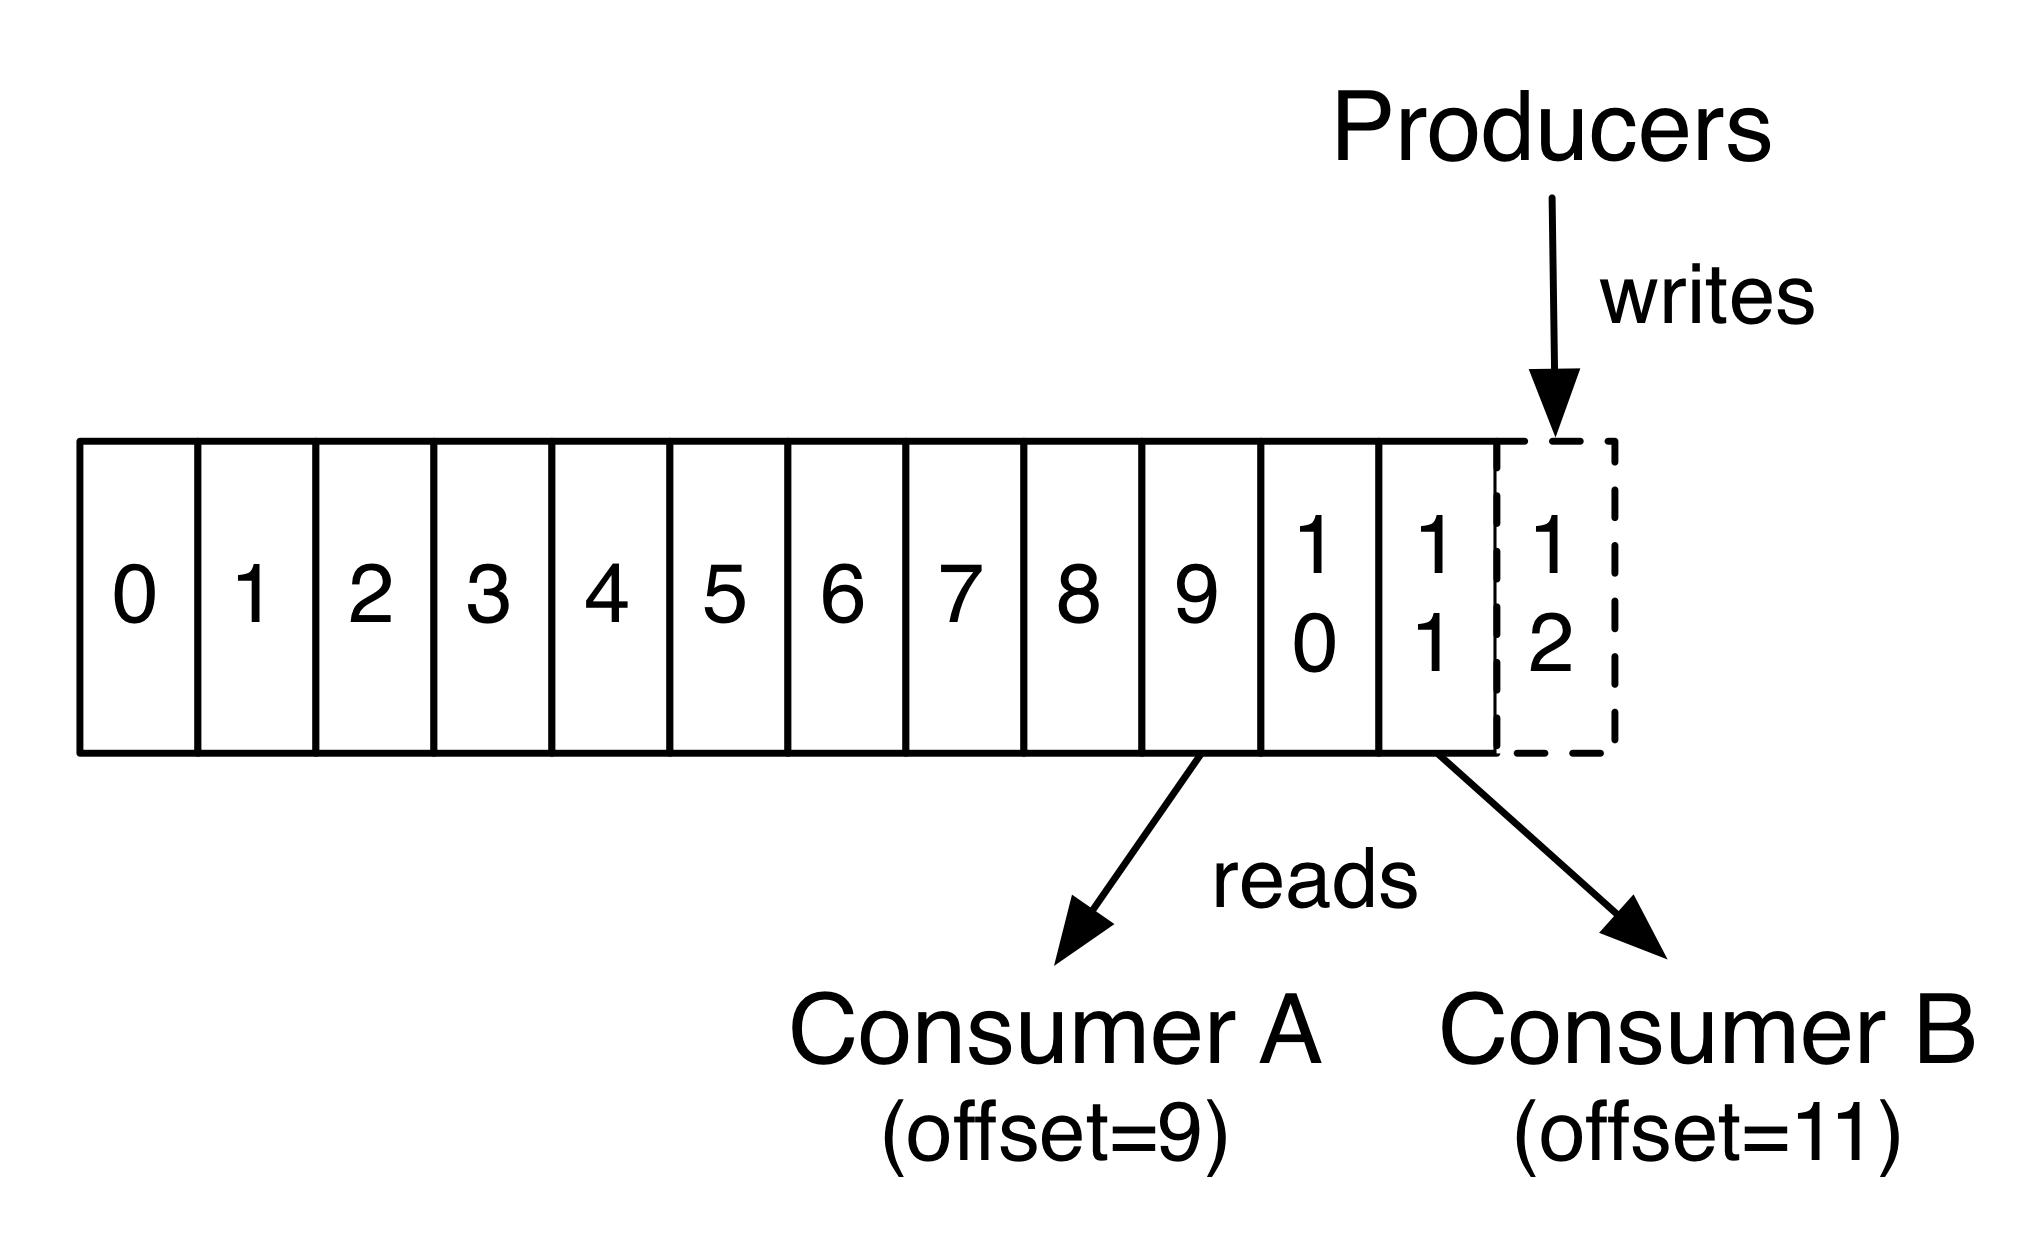
\includegraphics{img/kafka-topic-structure.png}
  \caption{Structure of records in a topic. Many producers can write to such topic and consumers can work with the records in arbitrary order.}
  \label{frameworks:kafka:topic}
\end{figure}

Figure \ref{frameworks:kafka:api} and next list taken from Kafka Framework documentation \citep{Kafka}
illustrates usage of four Kafka core client APIs:
\begin{itemize}
  \item The \textbf{Producer API} (see Section \ref{frameworks:kafka:producer}) allows an application to publish
    a stream of records to Kafka topics.
  \item The \textbf{Consumer API} (see Section \ref{frameworks:kafka:consumer}) allows an application to subscribe
    to topics and process the stream of records produced to them.
  \item The \textbf{Streams API} (see Section \ref{frameworks:kafka:streams}) allows an application to act as a stream processor,
    consuming an input stream from topics and producing an output stream to output topics,
    effectively transforming the input streams to output streams.
  \item The \textbf{Connector API} (see Section \ref{frameworks:kafka:connector}) allows building and running\break
    reusable producers or consumers
    that connect Kafka topics to existing applications or data systems.
    For example, a connector to a relational database might capture every change to a table. 
\end{itemize}

\begin{figure}[h]
  \center
  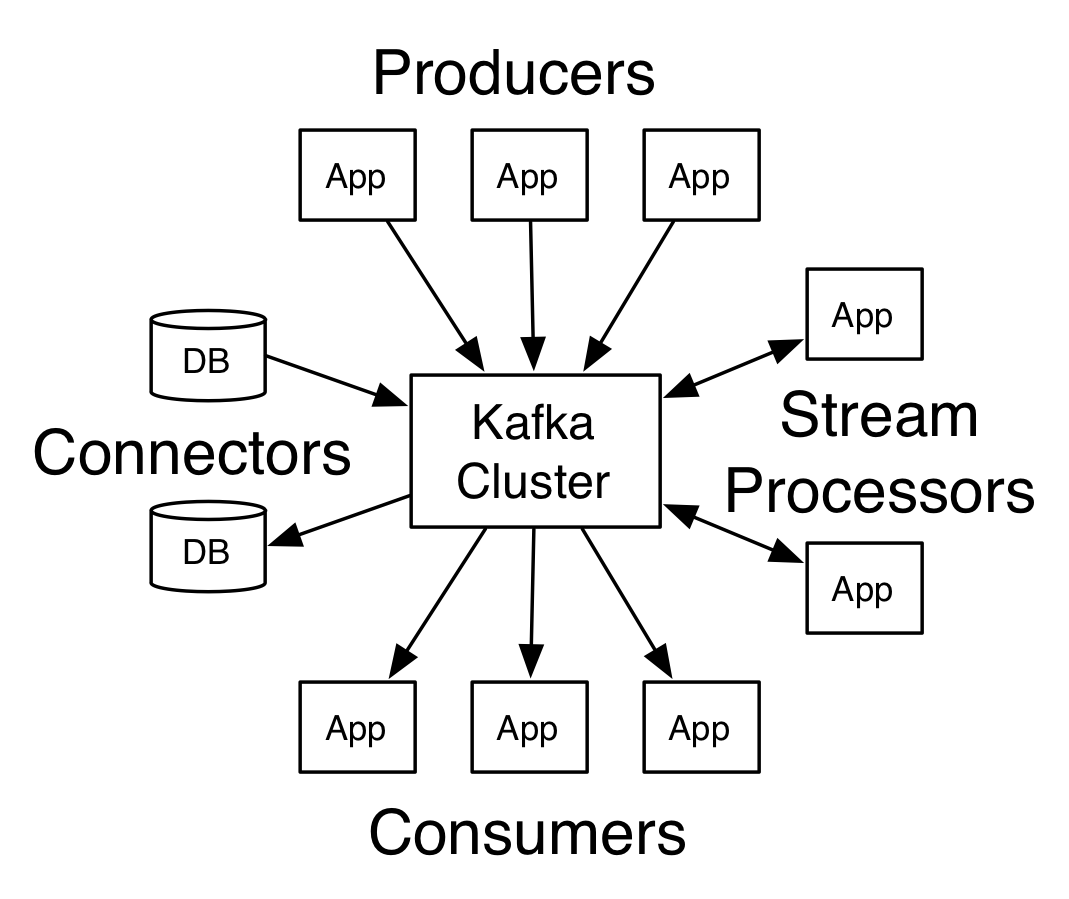
\includegraphics[width=100mm]{img/kafka-apis.png}
  \caption{Applications using differend kinds of Kafka APIs}
  \label{frameworks:kafka:api}
\end{figure}




\subsection{Producer API \label{frameworks:kafka:producer}}

Using Kafka Producer API, application can create new records and send them to topic of Kafka server.
It is illustrated by the example in Listing \ref{code:kafka:producer}.
We first configure \Code{KafkaProducer} and then we just send records to topic \Code{Topic}
to Kafka server by calling the \Code{send} method. Here we do not need to deal with the \Code{Serializer}s,
as they are provided for some basic Java classes (like \Code{String}) by framework itself.

\InsertCode{h}{code/kafka-producer}



\subsection{Consumer API \label{frameworks:kafka:consumer}}

Using Kafka Consumer API, application can handle new records that are arriving from server.
Listing \ref{code:kafka:producer} shows receiving such data.
We also configure \Code{KafkaConsumer} as in previous section.
On line \ref{code:kafka:consumer:subscribe} the program calls \Code{subscribe}
to register consumer to receive records in topic \Code{Topic}.
On line \ref{code:kafka:consumer:poll} server is queried for new data.
We use 1 second as maximal time limit, for which Kafka waits for new records to
arrive and then such records are returned and we can handle them.

\InsertCode{h}{code/kafka-consumer}



\subsection{Stream API \label{frameworks:kafka:streams}}

A Kafka Stream represents an unbounded, continuously updating data set.
It is an ordered, replayable, and fault-tolerant sequence of immutable data records.
Application defines its computational logic through processor topologies,
where processor topology is a graph of stream processors (nodes) that are
connected by streams (edges).

Stream processor is a node in the processor topology that represents
a processing step to transform data in streams by receiving one
input record at a time from its upstream processors in topology,
applying its operation on it and then produce one or more
output records to its downstream processors.

In topology, there are two special processors:

\begin{itemize}
  \item \textbf{Source Processor} is a stream processor
    that does not have any upstream processors. It produces an input stream
    to its topology from one or multiple Kafka topics by consuming records
    from these topics and forwarding them to its down-stream processors.
  \item \textbf{Sink Processor} is a stream processor
    that does not have down-stream processors. It sends any received records
    from its up-stream processors to a specified Kafka topic.
\end{itemize}

The way how topology can be defined is using the Kafka Streams Domain Specific Language (DSL).
It provides the most common data transformation operations, such as
\Code{map}, \Code{filter}, \Code{join} and \Code{aggregations}.
There exists also the low level Processor API that allows developers define
and connect custom processors and also interact with state stores.




\subsection{Connector API \label{frameworks:kafka:connector}}

A Kafka Connector is a tool for scalably and reliably streaming data between Kafka
and other systems. It makes it simple to quickly define connectors that move
large collections of data into and out of Kafka.
Kafka Connector can ingest entire databases or collect metrics from all
application servers into Kafka topics, making the data available
for stream processing with low latency.




\section{Requirements for Data Lineage Library \label{frameworks:requirements}}

In previous sections we demonstrated usage of different frameworks
that are usually used in Java applications to manipulate data.
We ignored their advanced features and showed some examples of reading
and writing data.

We described four types of data processing APIs / frameworks:
\begin{itemize}
  \item \textbf{JDBC API}, which is the Java API for working with SQL databases.
  \item \textbf{Spring JDBC Framework}, which simplifies the JDBC API.
  \item \textbf{MyBatis Framework}, which is the ORM framework.
  \item \textbf{Kafka Framework}, which is the distributed streaming platform.
\end{itemize}

Based on the overview of data processing frameworks,
in the rest of this section, we point out requirements on the library that
have to be fulfilled to successfully compute data lineage of applications,
where such frameworks are used for accessing the data.

\begin{enumerate}
  \item \textbf{Analysis of whole Java application.} \\
    The analysis should process whole application with all its dependencies.
  \item \textbf{Identifying the data sources and sinks.} \\
    The analysis should identify the places in application, where the data
    are read or written.
  \item \textbf{Correctness, accuracy and efficiency of computing data lineage.} \\
    The analysis should compute correct and accurate data lineage graphs in a reasonable time.
  \item \textbf{Work with external files.} \\
    The analysis should be able to handle not only Java classes,
    but also external files as many frameworks store their configuration
    outside of the code.
  \item \textbf{Use of concrete values.} \\
    The analysis should know the concrete values of Java primitives and\break
    \Code{String}s.
    This is necessary for identifying sources and sinks of data,
    such as files, database tables, etc.
  \item \textbf{Handle callbacks.} \\
    The analysis should work well with callbacks, as they are often
    used by frameworks to asynchronously notify application
    about some results of performed operation, or even
    to simplify the usage of other API.
  \item \textbf{Easy extendability.} \\
    The analysis need to be easily extended as new frameworks are developed
    and the core of symbolic analysis library needs to be prepared to add support for computing their data lineage.
\end{enumerate}



